Consider the Sine-Gordon equation on $\Omega \times I$, where $\Omega = [a,b]$ and $I = [0, T]$

\begin{align}
    &u_{tt} - u_{xx} + \sin{(u)} = 0, &&(x,t) \in \Omega \times I, \label{sine-gordon} \\
    &u(a,t) = f_1(t), \hspace{1mm} u(b,t) = f_2(t),  &&(x,t) \in \partial\Omega \times I,\label{sine-gordon-BC} \\
    &u(x,0) = u_0(x), \hspace{1mm} u_t(x,0) = u_1(x), &&x \in \Omega \times \{t=0\}. \label{sine-gordon-IC}
\end{align}

\subsubsection*{a)}

The analytical solution will be derived in the following. By introducing the change of variables $s = x - ct$, the equation \eqref{sine-gordon} can be expressed differently, because

\begin{equation*}
\begin{split}
    \frac{\partial u}{\partial t} &= \frac{\partial u}{\partial s}\frac{\partial s}{\partial t} = -c\frac{\partial u}{\partial s}, \\
    \frac{\partial^2 u}{\partial t^2} &= \frac{\partial }{\partial t}\left(-c\frac{\partial u}{\partial s}\right) = -c \frac{\partial }{\partial s}\frac{\partial u}{\partial t} = c^2 \frac{\partial^2 u}{\partial s^2}, \\
    \frac{\partial u}{\partial x} &= \frac{\partial u}{\partial s}\frac{\partial s}{\partial x} = \frac{\partial u}{\partial s}, \\
    \frac{\partial^2 u}{\partial x^2} &= \frac{\partial }{\partial x}\frac{\partial u}{\partial s} = \frac{\partial }{\partial s}\frac{\partial u}{\partial x} = \frac{\partial^2 u}{\partial s^2}. \\
\end{split}
\end{equation*}
This leads to the Sine-Gordon equation \eqref{sine-gordon} on the following form

\begin{equation*}
    \left(1-c^2\right)u_{ss} = \sin{(u)}.
\end{equation*}
Multiplying the equation by $u_s$ and performing integration by parts yields

\begin{align*}
    (1-c^2)\int u_{ss}u_s\mathrm{d}s &= (1-c^2)\left((u_{s})^2 - \int u_{ss}u_s\mathrm{d}s \right) + D_1\nonumber \\
    \implies (1-c^2)\int u_{ss}u_s\mathrm{d}s &= (1-c^2)\frac{1}{2}(u_{s})^2 + D_2, 
\end{align*}

where $D_2 = \frac{1}{2}D_1$, for the left hand side and 

\begin{equation*}
     \int \sin{(u)}u_s \mathrm{d}s = -\cos{(u)} + D_3,
\end{equation*}
for the right hand side. Hence, 

\begin{equation*}
    \frac{1}{2}(1-c^2)u^2_s = -\cos{(u)} + D, 
\end{equation*}
where $D = D_3 - D_2$. The constant $D$ determines one unique solution to the problem. Let $D = 1$ in this case. Thus, note that 

\begin{align*}
    u^2_s &= \frac{2(1 - \cos{(u)})}{(1-c^2)} \nonumber \\
    u^2_s &= \frac{4\sin^2{(\frac{u}{2})}}{(1-c^2)} \nonumber \\
    \frac{u_s}{\sin{(\frac{u}{2})}} &= \pm \frac{2}{\sqrt{1-c^2}}, 
\end{align*}
which, by integrating again, yields 

\begin{align*}
    &\frac{\mathrm{d}u}{\sin{(\frac{u}{2})}} = \pm \frac{2}{\sqrt{1-c^2}} \mathrm{d}s \nonumber \\
    &\mathrm{ln}\tan{\frac{u}{4}} = \pm \frac{s}{\sqrt{1-c^2}} + C \nonumber \\
    u(s) &= 4\arctan{\left(\exp{\left\{\pm \frac{s}{\sqrt{1-c^2}}\right\}}\right)},
\end{align*}
where the integration constant $C$ is set to 0. This means that one possible analytical solution to the Sine-Gordon equation \eqref{sine-gordon} is 

\begin{equation}
    u(x,t) = 4\arctan{\left(\exp{\left\{\pm \frac{x-ct}{\sqrt{1-c^2}}\right\}}\right)}, 
    \label{Part2-analytic-solution}
\end{equation}
when the integration constants are set to 0 and 1. 

\subsubsection*{b)} 
The following statement is proved in this section.
\begin{mydef}
The energy is conserved when $u_x(a,t) = u_x(b,t) = 0$.
\end{mydef}
\begin{proof}
The energy is the quantity that is obtained after multiplying equation \eqref{sine-gordon} by $u_t$ and integrating with respect to both $x$ and $t$. Before integrating, note the following equivalence relation

\begin{equation}
\begin{split}
    &u_tu_{tt} - u_tu_{xx} + u_t\sin{(u)} = 0 \\
    \iff &\frac{\partial}{\partial t}\left(\frac{1}{2}\left(\frac{\partial u}{\partial t}\right)^2 + \frac{1}{2}\left(\frac{\partial u}{\partial x}\right)^2 - \cos{(u)}\right) - \frac{\partial }{\partial x}\left(\frac{\partial u}{\partial t}\frac{\partial u}{\partial x}\right) = 0.
\label{part2b}
\end{split}
\end{equation}
This can be verified by noting that

\begin{equation*}
\begin{split}
    \frac{\partial}{\partial t}\left(\frac{1}{2}\left(\frac{\partial u}{\partial t}\right)^2 + \frac{1}{2}\left(\frac{\partial u}{\partial x}\right)^2 - \cos{(u)}\right) - \frac{\partial }{\partial x}\left(\frac{\partial u}{\partial t}\frac{\partial u}{\partial x}\right) &= 0, \\
    \frac{\partial^2 u}{\partial t^2}\frac{\partial u}{\partial t} + \frac{\partial^2 u}{\partial t \partial x}\frac{\partial u}{\partial x} + \frac{\partial u}{\partial t}\sin{(u)} - \left(\frac{\partial u}{\partial t}\frac{\partial^2 u}{\partial x^2} + \frac{\partial u}{\partial x}\frac{\partial^2 u}{\partial t\partial x}\right) &= 0.
\end{split}
\end{equation*}
Hence, integration of \eqref{part2b} yields

\begin{align}
    0 &=\int_0^{t'}\int_a^b\left(u_tu_{tt} - u_tu_{xx} + u_t\sin{(u)}\right)\mathrm{d}x\mathrm{d}t\nonumber \\
    &=\int_0^{t'} \int_a^b\left\{\frac{\partial}{\partial t}\left(\frac{1}{2}\left(\frac{\partial u}{\partial t}\right)^2 + \frac{1}{2}\left(\frac{\partial u}{\partial x}\right)^2 - \cos{(u)}\right) - \frac{\partial }{\partial x}\left(\frac{\partial u}{\partial t}\frac{\partial u}{\partial x}\right)\right\} \mathrm{d}x\mathrm{d}t, \nonumber \\
    &=\int_0^{t'}\int_a^b \frac{\partial}{\partial t}\left(\frac{1}{2}\left(\frac{\partial u}{\partial t}\right)^2 + \frac{1}{2}\left(\frac{\partial u}{\partial x}\right)^2 - \cos{(u)}\right)\mathrm{d}x\mathrm{d}t - \int_0^{t'}\int_a^b\frac{\partial }{\partial x}\left(\frac{\partial u}{\partial t}\frac{\partial u}{\partial x}\right)\mathrm{d}x\mathrm{d}t.
    \label{energyDoubleIntegration}
\end{align}
Note that

\begin{equation*}
    \int_a^b\frac{\partial }{\partial x}\left(\frac{\partial u}{\partial t}\frac{\partial u}{\partial x}\right)\mathrm{d}x = u_t(b,t^*)u_x(b,t^*)-u_t(a,t^*)u_x(a,t^*) = 0, 
\end{equation*}
when $u_x(b,t^*) = u_x(a,t^*) = 0, \hspace{1mm} \forall t^* \in I$ holds. This means that the second integral in equation \eqref{energyDoubleIntegration} evaluates to zero. Hence, the first integral must also evaluate to zero, which yields

\begin{equation*}
    \begin{split}
        0 &= \int_0^{t'}\int_a^b \frac{\partial}{\partial t} \left(\frac{1}{2}u_t^2 + \frac{1}{2}u_x^2 - \cos{(u)}\right)  \mathrm{d}x\mathrm{d}t \\
        &= \oint_\mathcal{C} \left(-\frac{1}{2}u_t^2 - \frac{1}{2}u_x^2 + \cos{(u)}\right)\mathrm{d}x \quad \text{(Green's Theorem)} \\
        &= -\left[ \int_a^b \left(-\frac{1}{2}u_t^2 - \frac{1}{2}u_x^2 + \cos{(u)}\right)\mathrm{d}x\right]_{t = t'} +  \left[ \int_a^b \left(-\frac{1}{2}u_t^2 - \frac{1}{2}u_x^2 + \cos{(u)}\right)\mathrm{d}x\right]_{t = 0} \\
        &= \left[ \int_a^b E_x\mathrm{d}x\right]_{t = t'} - \left[ \int_a^b E_x\mathrm{d}x\right]_{t = 0} \\
        &= E(t') - E(0), 
    \end{split}
\end{equation*}
where $E_x(x,t) := \frac{1}{2}u_t^2 + \frac{1}{2}u_x^2 - \cos{(u)}$, $E(t') := \left[ \int_a^b E_x\mathrm{d}x\right]_{t = t'}$ and $\mathcal{C}$ is the positively (anticlockwise) oriented boundary of the region $\{(x,t) \hspace{1mm} | \hspace{1mm} a \leq x \leq b, 0 \leq t \leq t' \}$. This shows that the energy $E$ is conserved, since $E(t') = E(0)$. 
\end{proof}

In the literature, e.g. \cite{SG-energy}, the energy density is usually defined as $E_x(x,t) = \frac{1}{2}u_t^2 + \frac{1}{2}u_x^2 + 1 - \cos{(u)}$. This does not contradict our derivation, because an arbitrary constant could have been included inside the parenthesis in the equivalence relation \eqref{part2b}. Therefore, this convention will be used in the following, in order to ensure that the energy is a positive quantity. 

\begin{comment}
% Siste linje du hadde ovenfor, Jim, i tilfelle du vil ha den.
&= \left[-\frac{1}{2}(\|u_t\|^2_{L_2} + \|u_x\|^2_{L_2}) + \int_a^b \cos{u} \mathrm{d}x\right]_{t = t}  + \left[-\frac{1}{2}(\|u_t\|^2_{L_2} + \|u_x\|^2_{L_2}) + \int_b^a \cos{u} \mathrm{d}x\right]_{t = 0}
\end{comment}

\begin{comment}
\textcolor{blue}{Jostein sitt forslag til hva som kan stemme; Jeg tror ikke energien er hele likningen integrert for da hadde den vært null hele tiden.}

From the equation above \eqref{energyDoubleIntegration} we find that
\begin{equation}
\begin{split}
    0 &= \frac{\mathrm{d}}{\mathrm{d}t} \int_0^t \int_a^b \left(\frac{1}{2}u_t^2 + \frac{1}{2}u_x^2 - \cos{u}\right)  \mathrm{d}x\mathrm{d}t = \frac{\mathrm{d}}{\mathrm{d}t} E(t),
\end{split}
\end{equation}
and hence the energy is a constant equal to its initial energy $E(t) = E(0)$. \textcolor{red}{Er nettopp dette jeg har prøvd å vise også :) Hvordan vet du at $E(t)$ er hele dette integralet?} \textcolor{green}{Jim: Står det ikke noe på piazza om at man skal komme fram til et uttrykk uten integraltegn?} \textcolor{blue}{Jo, det står, men vi vet jo fortsatt ikke hvordan E(t) er definert, så det hjelper jo ikke så veldig mye...}
\end{comment}

\subsubsection*{c)}
The Sine-Gordon equation \eqref{sine-gordon} is discretized using the principle of semi-discretization \cite{Owren}. Two systems of ODEs are developed; one with first order and one with second order in time.

\begin{comment}
To begin with, the domain $\Omega \times I$ is discretized along the $x$- and $t$-directions in the following way
\begin{equation*}
\begin{split}
    &x_0 = a \text{,} \hspace{2mm} x_1 = a+\frac{b-a}{M+1} \text{,} \hspace{2mm} \dots \text{,} \hspace{2mm} x_M = a+\frac{M(b-a)}{M+1} \text{,} \hspace{2mm} x_{M+1} = b, \\
    &t_0 = 0 \text{,} \hspace{2mm} t_1 = \frac{T}{N} \text{,} \hspace{2mm} \dots \text{,} \hspace{2mm} t_{N-1} = \frac{T(N-1)}{N} \text{,} \hspace{2mm} t_{N} =T.
\end{split}
\end{equation*}
Let $h = \frac{b-a}{M+1}$ and $k=\frac{T}{N}$.
\end{comment}
To begin with, the $x$-axis is discretized in the following manner

\begin{equation*}
    x_0 = a \text{,} \hspace{2mm} x_1 = a+\frac{b-a}{M+1}, \ldots , x_M = a+\frac{M(b-a)}{M+1},  x_{M+1} = b,
\end{equation*}
letting $h = \frac{b-a}{M+1}$.
A central finite difference approximation is used to discretize the spatial derivative. Let $u_m := u(x_m, t)$. The stencil is then on the form 

\begin{equation*}
    (u_m)_{xx} = \frac{1}{h^2} \delta^2 u_m = \frac{1}{h^2}(u_{m-1} - 2u_m + u_{m+1}) + \mathcal{O}(h^2), \quad 1 \le m \le M, 
\end{equation*}
%where $x_m=a+m h$ and $t_n=n k$ are on the grid defined earlier. 
\noindent Inserting the stencil for the spatial derivative into the Sine-Gordon equation \eqref{sine-gordon} gives

\begin{equation*}
    \ddot{u}_m = \frac{1}{h^2}\delta^2u_m - \sin{(u_m)} + \mathcal{O}(h^2),
\end{equation*}
where the quantity $\ddot{u}_m$ denotes the second order derivative of $u_m$ with respect to time. Note that this is a set of ordinary differential equations (ODE) along lines parallel to the $t$-axis and across the $x$-axis at the grid points $x_m$. Next, the approximate solutions $v_m := v_m(t) \approx u_m(t)$ are introduced, where the truncation error is neglected, by requiring that 

\begin{equation*}
    \ddot{v}_m = \frac{1}{h^2}\delta^2 v_m - \sin{(v_m)} \text{,} \hspace{2mm} 1 \le m \le M.
\end{equation*} 
Considering the Dirichlet boundary conditions \eqref{sine-gordon-BC}, namely that $u(a,t) = v_0(t) = f_1(t)$ and $u(b,t)=v_{M+1}(t)= f_2(t)$, the ODEs can be reformulated in the following manner

\begin{equation}
    \boldsymbol{\ddot{v}} = \frac{1}{h^2} 
    \begin{pmatrix}
    -2 & 1 & 0 & \dots & 0\\
    1 & -2 & 1 & 0 & \dots \\
    \ddots & \ddots & \ddots & \ddots &\ddots \\
    0 & \dots & 1 & -2 & 1 \\
    0 & \dots & 0 & 1 & -2 \\
    \end{pmatrix}
    \boldsymbol{v} + 
    \begin{pmatrix}
    \frac{1}{h^2} f_1(t) - \sin{(v_1)} \\
    -\sin{(v_2)} \\
    \vdots \\
    -\sin{(v_{M-1})} \\
    \frac{1}{h^2} f_2(t) - \sin{(v_M)}\\
    \end{pmatrix} %\text{,} \hspace{2mm} 0 \leq n \leq N
    \label{part2cFirstSystem}
\end{equation}

\noindent where $\boldsymbol{v} = [v_1,v_2,\dots,v_M]^T$ and $\boldsymbol{\ddot{v}} = [\ddot{v}_1,\ddot{v}_2,\dots,\ddot{v}_M]^T$. In compact notation, the system of equations \eqref{part2cFirstSystem} can be written as

\begin{comment}
Note that the boundary functions are evaluated in continuous time, and not with $t=t_n$ on the grid defined earlier. This is because, later, when using ODE-solvers defined below, the system can be dependent of time and this proves therefore to be more accurate \textcolor{red}{Dobbelsjekke dette. Utdype kanskje?} \textcolor{blue}{Ja, det kan være en idé. Ikke helt sikker på hva dette betyr akk nå, men det blir kanskje klarere jo lenger jeg leser :) t-aksen blir jo diskretisert når metodene brukes i praksis uansett?}. 
\end{comment}

\begin{equation}
    \label{SG-disc_2nd_order_in_time}
    \boldsymbol{\ddot{v}} = \frac{1}{h^2}A\boldsymbol{v} + \boldsymbol{g}(t, \boldsymbol{v}). %\text{,} \hspace{2mm} 0 \leq n \leq N.
\end{equation}

\noindent This is a system of equations of second order in time and will be used later, in combination with Runge-Kutta-Nyström methods defined in \textbf{e)}, to solve the Sine-Gordon equation numerically.

By introducing $\boldsymbol{w}=\boldsymbol{\dot{v}}$ and the vector $\boldsymbol{y}=[\boldsymbol{v}^T,\boldsymbol{w}^T]^T$, \eqref{SG-disc_2nd_order_in_time} can be reformulated to a first order system of differential equations in time:

\begin{equation}
    \dot{\boldsymbol{y}} = \begin{pmatrix}
    \boldsymbol{\dot{v}} \\
    \boldsymbol{\dot{w}} \\
    \end{pmatrix}
    = \begin{pmatrix}
    \boldsymbol{w} \\
    \frac{1}{h^2}A\boldsymbol{v} + \boldsymbol{g}(t, \boldsymbol{v})\\
    \end{pmatrix}. %\text{,} \hspace{2mm} 0 \leq n \leq N.
    \label{SG-disc_1st_order_in_time}
\end{equation}

\noindent This system of equations will be used in combination with Runge-Kutta methods defined in \textbf{d)} to find numerical solutions to the Sine-Gordon equation.

\subsubsection*{d)}
Runge-Kutta (RK) integrators can be used to solve an initial value problem on the form
\begin{equation}
    \dot{\boldsymbol{y}} = f(t,\boldsymbol{y}) \text{,} \hspace{2mm} \boldsymbol{y}(t_0) = \boldsymbol{y}^0. \nonumber
\end{equation}
Comparing with the system of equations \eqref{SG-disc_1st_order_in_time} and using the initial conditions \eqref{sine-gordon-IC} yields

\begin{equation*}
    \dot{\boldsymbol{y}} = \begin{pmatrix}
    \boldsymbol{w} \\
    \frac{1}{h^2}A\boldsymbol{v} + \boldsymbol{g}(t,\boldsymbol{v})
    \end{pmatrix} =: F(t,\boldsymbol{y}) \text{,} \hspace{2mm} \boldsymbol{y}(0) = \boldsymbol{y}^0 = \begin{pmatrix}
    \boldsymbol{v}^0\\
    \boldsymbol{w}^0
    \end{pmatrix},
\end{equation*}
where $\boldsymbol{v}^0 = \boldsymbol{v}|_{t=0} = [u_0(x_1), \ldots, u_0(x_M)]^T$, and similarly $\boldsymbol{w}^0 = \boldsymbol{w}|_{t=0} = [u_1(x_1), \ldots, u_1(x_M)]^T$, where $u_0(x) = u(x, 0)$ and $u_1(x) = u_t(x, 0)$.

The explicit Runge-Kutta methods RK2, RK3 and RK4 are used in our implementation. It is given that these methods are of second, third and fourth order, in accordance with their names. This means that the total accumulated error after using the iterative method along the time grid is of order $\mathcal{O}(k^2)$, $\mathcal{O}(k^3)$ and $\mathcal{O}(k^4)$ for the RK2, RK3 and RK4 methods respectively. Let $\boldsymbol{Y}^n \approx \boldsymbol{y}(t_n)$ be the numerical solutions produced by the integrators at time $t=t_n$. A step with the explicit RK2 method takes the form

\begin{equation*}
    \begin{split}
        &s_1 = F(t,\boldsymbol{Y}^n) \\
        &s_2 = F(t+k,\boldsymbol{Y}^n+k s_1)\\
        \boldsymbol{Y}^{n+1} &= \boldsymbol{Y}^n + \frac{k}{2}\left(s_1+s_2\right),
    \end{split}
\label{RK2-method}
\end{equation*}

\noindent where the calculations are repeated iteratively for $0 \leq n \leq N-1$. The iterative scheme is run until $t_N=T$, so the step length in the time direction may be defined as $k=\frac{T}{N}$. Similarly, a step with the RK3 and RK4 methods take the form

%\begin{equation*}
%\begin{aligned}
%    &\text{RK3}   &    & \text{RK4} \\
%    &s_1 = F(t,Y^n)  &   &s_1 = F(t,Y^n) \\
%    &s_2 = F(t+\frac{k}{2},Y^n + \frac{k}{2}s_1) &   &s_2 = F(t+\frac{k}{2},Y^n+\frac{k}{2}s_1) \\
%    &s_3 = F(t+k,Y-k s_1 + 2k s_2) &  &s_3 = F(t + \frac{k}{2}, Y^n + \frac{k}{2}s_2) \\
%    &     &    & s_4 = F(t+k,Y^n+k s_3)  \\
%    Y^{n+1} &= Y^n + \frac{k}{6}\left(s_1 + 4s_2 +  s_3\right)   &  Y^{n+1} &= Y^n + \frac{k}{6} \left(s_1+2s_2+2s_3+s_4\right).
%    \label{RK_3&4}
%\end{aligned}
%\end{equation*}

\setlength{\arrayrulewidth}{0.5mm}
\setlength{\tabcolsep}{18pt}
\renewcommand{\arraystretch}{2.3}
\begin{center}
    \begin{tabular}{ |c | c| }
          \hline			
          RK3 & RK4 \\
          \hline
          $s_1 = F(t,\boldsymbol{Y}^n)$  &   $s_1 = F(t,\boldsymbol{Y}^n)$ \\
          $s_2 = F(t+\frac{k}{2}, \boldsymbol{Y}^n + \frac{k}{2}s_1)$ &   $s_2 = F(t+\frac{k}{2}, \boldsymbol{Y}^n+\frac{k}{2}s_1)$ \\
    $s_3 = F(t+k,\boldsymbol{Y}^n-k s_1 + 2k s_2)$ & $s_3 = F(t + \frac{k}{2}, \boldsymbol{Y}^n + \frac{k}{2}s_2)$ \\
         &    $s_4 = F(t+k,\boldsymbol{Y}^n+k s_3)$  \\
          \hline
          $\boldsymbol{Y}^{n+1} = \boldsymbol{Y}^n + \frac{k}{6}\left(s_1 + 4s_2 +  s_3\right)$ & $\boldsymbol{Y}^{n+1} = \boldsymbol{Y}^n + \frac{k}{6} \left(s_1+2s_2+2s_3+s_4\right)$. \\
         \hline
    \end{tabular}
\end{center}

In order to perform $h$- and $k$-refinement?, the analytical solution, as well as a domain, needs to be specified for the three RK-integrators. The analytical solution is chosen to be equation \eqref{Part2-analytic-solution} with a minus sign in the exponential function. Moreover, the constant in the change of variables is set to $c=\frac{1}{2}$. Furthermore, the domain that is studied is $\Omega \times I = [-5,5] \times [0,5]$. Hence, the analytical solution is

\begin{equation}
    u(x,t) = 4\arctan{\left(\exp{\left\{-\frac{2x-t}{\sqrt{3}}\right\}}\right)},
    \label{Part2-analytic-solution-specified}
\end{equation}
and the associated boundary and initial conditions \eqref{sine-gordon-BC}
and \eqref{sine-gordon-IC} now become

\begin{equation}
\begin{aligned}
\label{Part2-specified-BC&IC_d&e}
    f_1(t) &= 4\arctan{\left(\exp{\left\{\frac{10+t}{\sqrt{3}}\right\}}\right)},  & f_2(t) & = 4\arctan{\left(\exp{\left\{-\frac{10-t}{\sqrt{3}}\right\}}\right)}, \\
    u_0(x) &= 4\arctan{\left( \exp{\left\{-\frac{2x}{\sqrt{3}}\right\}} \right)},  & u_1(x) &= \frac{4\exp{\left\{- \frac{2x}{\sqrt{3}}\right\}}}{\sqrt{3}\left(1 + \exp{\left\{- \frac{4x}{\sqrt{3}} \right\}} \right)}.
\end{aligned}
\end{equation}

\begin{figure}[t]
    \centering
    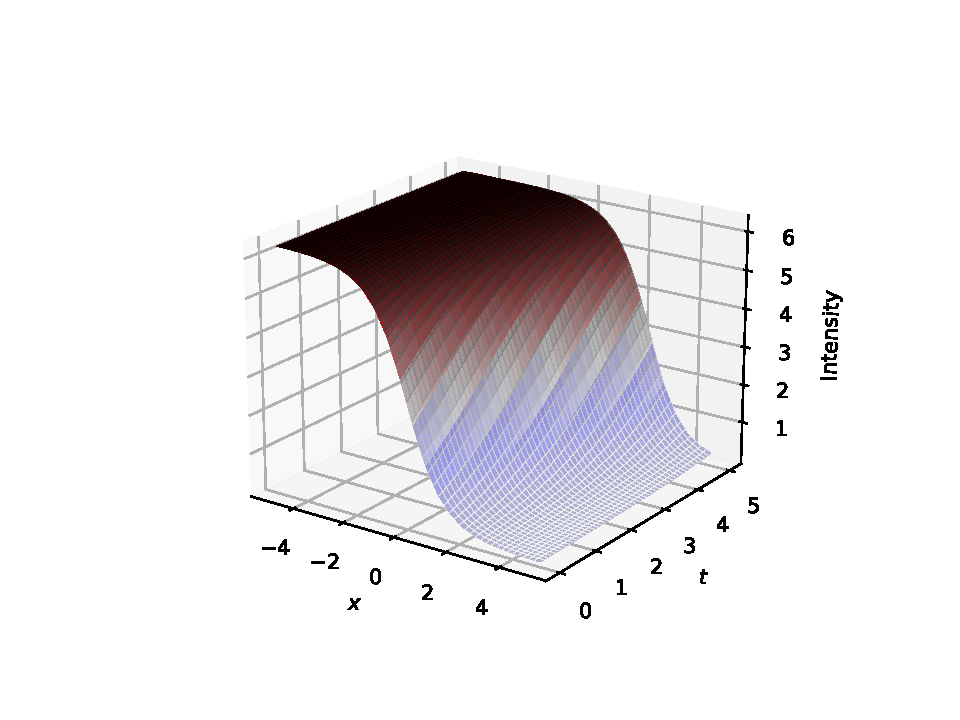
\includegraphics[width = 0.85\linewidth]{plots/part2d_sol.pdf}
    \caption{Sine-Gordon equation solved on $x \in [-5,5]$ and $t \in [0,5]$ with Dirichlet boundary conditions and initial condition $u(x,0)=4\arctan{\left( \exp{\left\{-\frac{2x}{\sqrt{3}}\right\}} \right)}$. The numerical solution is calculated using RK4 with $M=N=20$ and plotted in a \textit{seismic} color map. The analytical solution is plotted in grey.}
    \label{fig:part2d_sol}
\end{figure}

The numerical and analytical solution \eqref{Part2-analytic-solution-specified} to the Sine-Gordon equation is shown in figure \ref{fig:part2d_sol}. Here, the numerical solution is calculated using the RK4-method on a mesh grid of low resolution. 

Next, $h$- and $k$-refinement for the three Runge-Kutta integrators is considered. Due to the CFL-condtition, there is a constraint on the fraction $k/h$. The constraint depends on the chosen integrator. The constraint prevents us from performing $k$-refinement in the usual way by setting $M$ to a large value and increasing $N$ from a small value. To avoid this problem, a reference solution is used, namely a numerical solution calculated in the same manner, but with parameters $M_{ref}$ and $N_{ref}$. Note that this reference solution replaces the analytical solution when computing the relative error. The refinement along the time direction is thus performed by finding numerical solutions with $M=M_{ref}$ and increasing $N$ while ensuring that $N<<N_{ref}$. Then, the relative error with respect to the reference solution can be computed. We set $M=M_{ref}$ so that the error along the $x$-axis for the numerical solutions and the reference solution cancel each other out. This way, the observed error is a consequence of error in time and the CFL-condition is still fulfilled, which means that the solutions are stable. This approach is similar to what has been done in \cite{LOVE201333}. The plot of the $k$-refinement, with $M_{ref}=400, N_{ref}=10000$, is shown in figure \ref{fig:part2d_RK_tref} for all the three Runge-Kutta integrators. As is apparent, the relative errors match the expected orders for all three methods. More specifically, the relative error decreases as $\mathcal{O}(k^2)$, $\mathcal{O}(k^3)$ and $\mathcal{O}(k^4)$ for the RK2, RK3 and RK4 methods respectively. 

\begin{figure}
\centering
\subfloat[$h$-refinement]{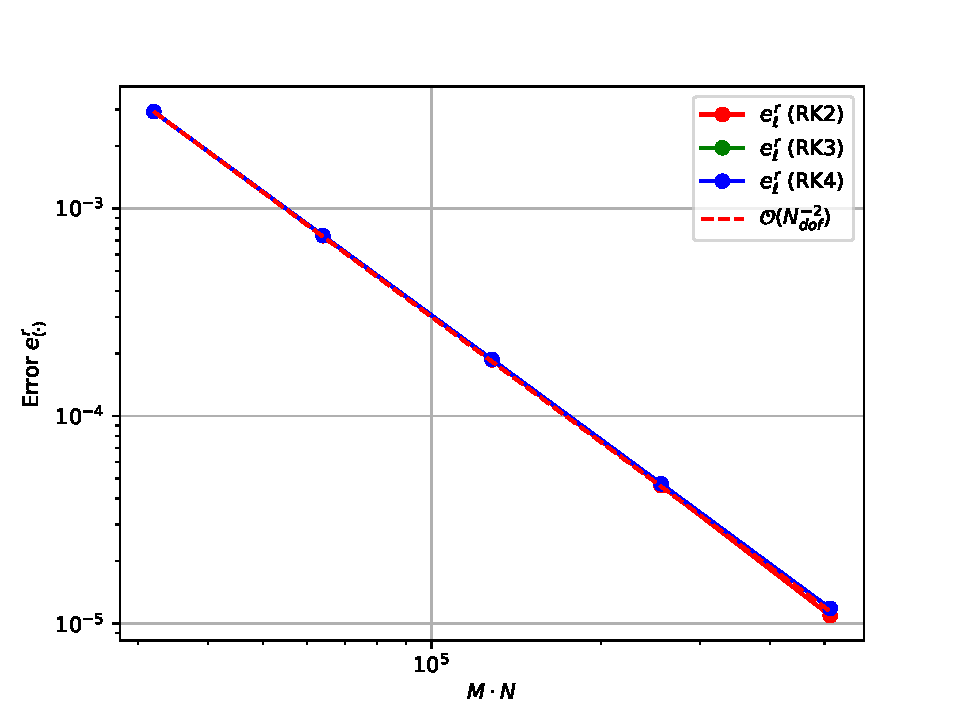
\includegraphics[width=0.9\linewidth]{plots/part2_RK_href.pdf}\label{fig:part2d_RK_href}}\hspace{0mm}
\subfloat[$k$-refinement]{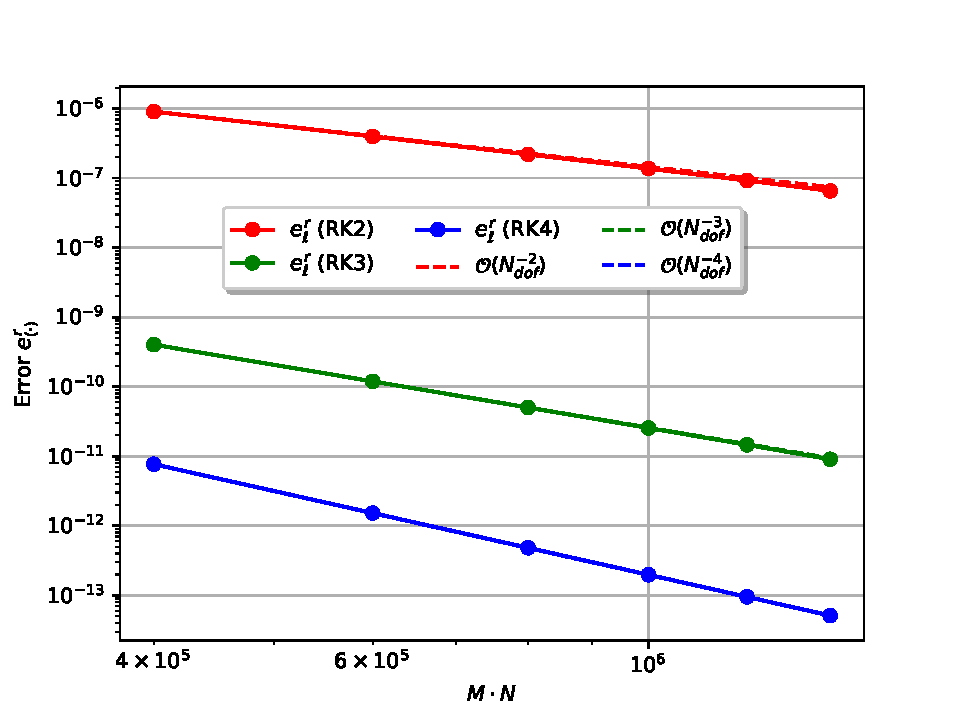
\includegraphics[width=0.85\linewidth]{plots/part2_RK_tref.pdf}\label{fig:part2d_RK_tref}}\hspace{0mm}
\caption{Sine-Gordon equation solved on $x \in [-5,5]$ and $t \in [0,5]$ with Dirichlet boundary conditions and initial condition $u(x,0)=4\arctan{\left( \exp{\left\{-\frac{2x}{\sqrt{3}}\right\}} \right)}$. The relative error obtained with $h$-refinement and $N=1000$ is plotted in (a), while the relative error obtained with $k$-refinement and $M_{ref}=400, N_{ref}=10000$ is plotted in (b). This is done for the different Runge-Kutta integrators in both cases.}
\end{figure}

\begin{comment}
Consider the PDE $f_t + a f_x = 0$. The CFL-condition states that for the numerical solution of this equation to converge, $|a|\frac{k}{h} \le 1$ must be satisfied \cite{Owren}. The sine-Gordon equation can be written in this format as
\end{comment}

The $h$-refinement is executed in the usual manner, i.e. the relative error is calculated with respect to the analytical solution \eqref{Part2-analytic-solution-specified}. Figure \ref{fig:part2d_RK_href} shows a plot of the $h$-refinement for all the Runge-Kutta integrators. Since the central difference approximation is used along the $x$-axis when deriving the difference scheme, second order convergence of the relative error for all the Runge-Kutta methods is expected. As seen in the figure, the results from the implementation match these expectations.  

\subsubsection*{e)}
Runge-Kutta-Nyström (RKN) integrators can be used to solve initial value problems of second-order ODE's on the form

\begin{equation*}
    \ddot{y} = f(t,y,\dot{y}) \text{,} \hspace{2mm} y(t_0) = y^0 \text{,} \hspace{2mm} \dot{y}(t_0) = \dot{y}^0. 
\end{equation*}
In our case, we have the second-order ODE

\begin{equation*}
\begin{split}
    \boldsymbol{\ddot{v}} &= \frac{1}{h^2}A\boldsymbol{v} + \boldsymbol{g}(t,\boldsymbol{v}) := G(t,\boldsymbol{v}),\\ &\boldsymbol{v}|_{t=0}=\boldsymbol{v}^0 \text{,} \hspace{2mm} \boldsymbol{\dot{v}}|_{t=0} = \boldsymbol{\dot{v}}^0,
\end{split}
\end{equation*}
where the initial conditions are $\boldsymbol{v}^0 = [u_0(x_1), \ldots, u_0(x_M)]^T$ and $\boldsymbol{\dot{v}}^0 = [u_1(x_1), \ldots, u_1(x_M)]^T$.

In our implementation, the explicit and symplectic integrators RKN-12 and RKN-34 are used. It is given that RKN-12 is a method of second order and the RKN-34 is a fourth order method, which means that their total accumulated error is of order $\mathcal{O}(k^2)$ and $\mathcal{O}(k^4)$ respectively. Let $\boldsymbol{V}^n \approx \boldsymbol{v}(t_n)$ and $\dot{\boldsymbol{V}}^n \approx \dot{\boldsymbol{v}}(t_n)$ be the numerical solutions produced by the integrators at time $t = t_n$. The RKN-12 algorithm takes the form    

\begin{equation*}
\begin{split}
    &s_1 = G(t_n,\boldsymbol{V}^n) \\
    \dot{\boldsymbol{V}}^{n+1} &= \dot{\boldsymbol{V}}^n + k s_1 \\
    \boldsymbol{V}^{n+1} &= \boldsymbol{V}^n + k\dot{\boldsymbol{V}}^n + k^2 \frac{s_1}{2},
\end{split}
\end{equation*}
and, similarly, the RKN-34 algorithm looks like

\begin{comment}
\begin{equation*}
\begin{split}
    &s_1 = G(t_n,\boldsymbol{v}) \\
    \boldsymbol{\dot{v}}^{n+1} &= \boldsymbol{\dot{v}}^n + k s_1 \\
    \boldsymbol{v}^{n+1} &= \boldsymbol{v}^n + k\boldsymbol{\dot{v}}^n + k^2 \frac{s_1}{2},
\end{split}
\end{equation*}
\end{comment}


\begin{equation*}
    \begin{split}
        &s_1 = G\left(t_n+(\frac{1}{2}-\delta)k,\boldsymbol{V}^n+(\frac{1}{2}-\delta)k\dot{\boldsymbol{V}}^n\right)\\
        &s_2 = G\left(t_n+\frac{k}{2},\boldsymbol{V}^n+\frac{k}{2} \dot{\boldsymbol{V}}^n + \frac{k^2}{24\delta} s_1\right)\\
        &s_3 = G\left(t+(\frac{1}{2}+\delta)k, \boldsymbol{V}^n+(\frac{1}{2}+\delta)k\dot{\boldsymbol{V}}^n + k^2(\frac{1}{12\delta}s_1 + (\delta-\frac{1}{12\delta})s_2)\right)\\
        \dot{\boldsymbol{V}}^{n+1} &= \dot{\boldsymbol{V}}^n + k\left(\frac{s_1+s_3}{24\delta^2} + (1-\frac{1}{12\delta^2})s_2\right) \\
        \boldsymbol{V}^{n+1} &= \boldsymbol{V}^{n} + k\dot{\boldsymbol{V}}^n + k^2\left( (\frac{1}{48\delta^2}+\frac{1}{24\delta})s_1+ (\frac{1}{2}-\frac{1}{24\delta^2})s_2 + (\frac{1}{48\delta^2}-\frac{1}{24\delta})s_3\right),
    \end{split}
\end{equation*}

\begin{comment}
\begin{equation*}
    \begin{split}
        &s_1 = G\left(t+(\frac{1}{2}-\delta)k,\boldsymbol{v}^n+(\frac{1}{2}-\delta)k\boldsymbol{\dot{v}}^n\right)\\
        &s_2 = G\left(t+\frac{k}{2},\boldsymbol{v}^n+\frac{k}{2}\boldsymbol{\dot{v}}^n + \frac{k^2}{24\delta} s_1\right)\\
        &s_3 = G\left(t+(\frac{1}{2}+\delta)k,\boldsymbol{v}^n+(\frac{1}{2}+\delta)k\boldsymbol{\dot{v}}^n + k^2(\frac{1}{12\delta}s_1 + (\delta-\frac{1}{12\delta})s_2)\right)\\
        \boldsymbol{\dot{v}}^{n+1} &=\boldsymbol{\dot{v}}^n + k\left(\frac{s_1+s_3}{24\delta^2} + (1-\frac{1}{12\delta^2})s_2\right) \\
        \boldsymbol{v}^{n+1} &= \boldsymbol{v}^n + k\boldsymbol{\dot{v}}^n + k^2\left( (\frac{1}{48\delta^2}+\frac{1}{24\delta})s_1+ (\frac{1}{2}-\frac{1}{24\delta^2})s_2 + (\frac{1}{48\delta^2}-\frac{1}{24\delta})s_3\right),
    \end{split}
\end{equation*}
\end{comment}
where the generating coefficient is $\delta = \frac{1}{12}(2-\sqrt[3]{4}-\sqrt[3]{16})$, not to be confused with the central difference operator. These calculations will be executed iteratively for $0 \leq n \leq N-1$. 

\begin{figure}
\centering
\subfloat[$h$-refinement]{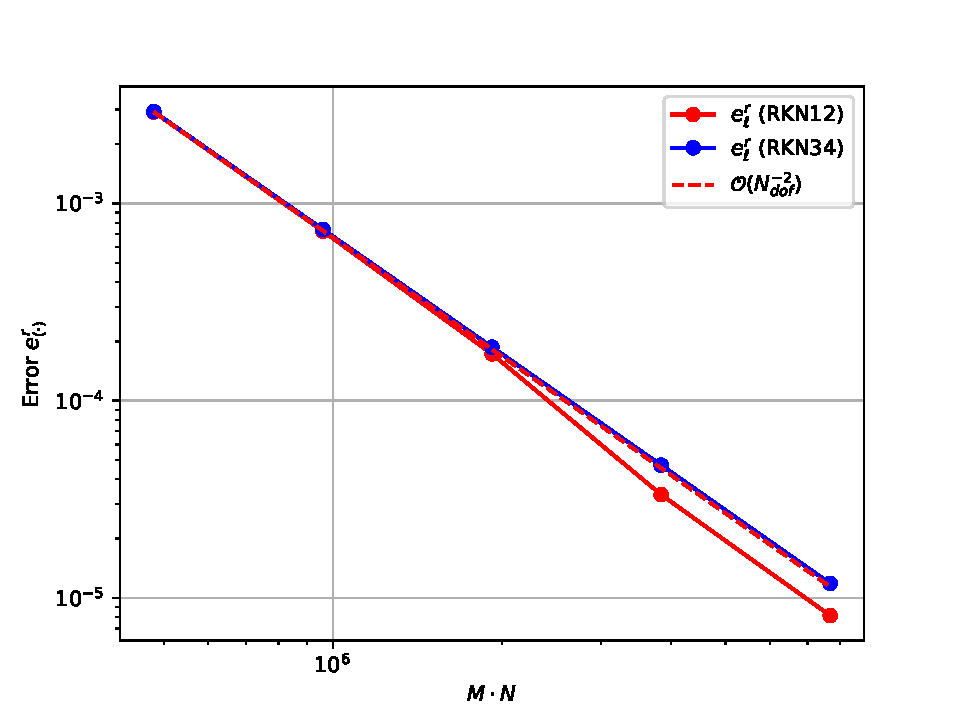
\includegraphics[width=0.9\linewidth]{plots/part2_RKN_href.pdf}\label{fig:part2e_RKN_href}}\hspace{0mm}
\subfloat[$k$-refinement]{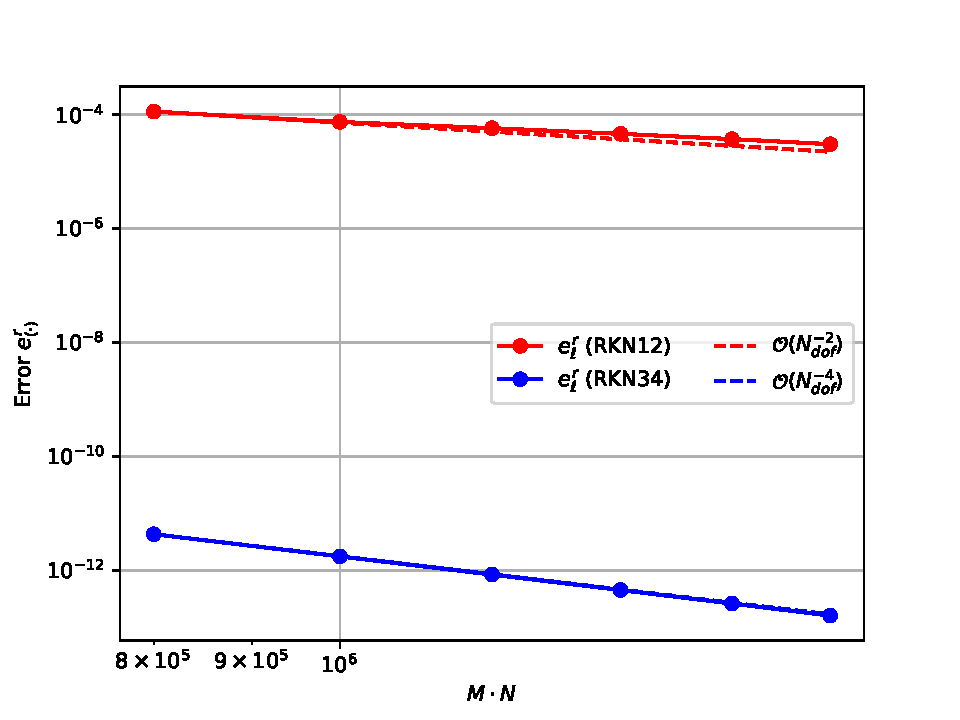
\includegraphics[width=0.85\linewidth]{plots/part2_RKN_tref.pdf}\label{fig:part2e_RKN_tref}}\hspace{0mm}
\caption{Sine-Gordon equation solved on $x \in [-5,5]$ and $t \in [0,5]$ with Dirichlet boundary conditions and initial condition $u(x,0)=4\arctan{\left( \exp{\left\{-\frac{2x}{\sqrt{3}}\right\}} \right)}$. The relative error obtained with $h$-refinement and $N=15000$ is plotted in (a), while the relative error obtained with $k$-refinement and $M_{ref}=400, N_{ref}=10000$ is plotted in (b). This is done for RKN-12 and RKN-34 in both cases.}
\end{figure}

The same problem as in \textbf{d)} arises when executing $k$-refinement. By performing the $k$-refinement as explained in \textbf{d)}, with $M_{ref}=400, N_{ref}=10000$, it is observed that the relative error using the RKN-34 integrator decreases with $\mathcal{O}(k^4)$ and the error with the RKN-12 integrator is of order $\mathcal{O}(k^2)$, which is precisely as expected. This can be seen in figure \ref{fig:part2e_RKN_tref}. 

The $h$-refinement plots with the RKN integrators are shown in figure \ref{fig:part2e_RKN_href}. The relative error is, as in \textbf{d)}, calculated with respect to the analytical solution. As expected, due to the central difference approximation, the relative error decreases in order $\mathcal{O}(h^2)$. Furthermore, it can be observed that the relative error with the RKN-12 method seems to be unstable for large values of $M$. We have observed that the RKN-12 integrator has a very strict CFL-condition, i.e. it needs a large $N$. In this case, the $h$-refinement is calculated with $N=15000$, while in \textbf{d)} it was sufficient to let $N=1000$. If $N$ is chosen a lot smaller will the graph for RKN-12, shown in figure \ref{fig:part2e_RKN_href}, deviate from the expected curve. 

\subsubsection*{f)}

Consider the boundary value problem (BVP)

\begin{align}
    &u_{tt} - u_{xx} + \sin{(u)} = 0, &&(x,t) \in \Omega \times I,  \\
    &u(-2,t) = 0, \hspace{1mm} u(2,t) = 0,  &&(x,t) \in \partial\Omega \times I, \\
    &u(x,0) = \sin{(\pi x)^2e^{-x^2}}, &&x \in \Omega \times \{t=0\}, \\
    &u_t(x,0) = \sin{(\pi x)^4e^{-x^2}}, &&x \in \Omega \times \{t=0\}, 
\end{align}
where $\Omega = [-2, 2]$ and $I = [0,4]$. The RK4 and RKN-34 integrators are applied, in order to approximate the solution of the BVP. The numerical solution is shown in three dimensions in figure \ref{fig:part2f_3d_plott}. Figure \ref{fig:part2f_sol} shows the numerical solution in the $x-z$-plane, at different times. Here, it is observed that the solution is anti-symmetric at $t=4$ in relation to its initial condition.

\begin{figure}
\centering
\subfloat[3d-plot of numerical solution]{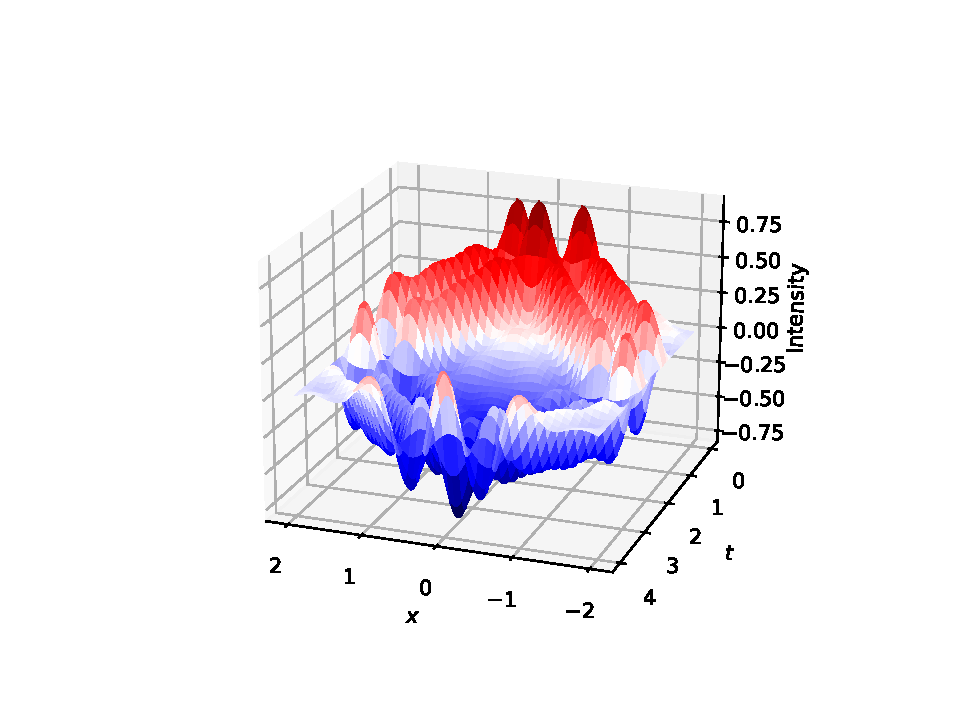
\includegraphics[width=0.9\linewidth]{plots/part2f_3d_plott.pdf}\label{fig:part2f_3d_plott}}\hspace{0mm}
\subfloat[Numerical solution at $t=0$ and $t=4$.]{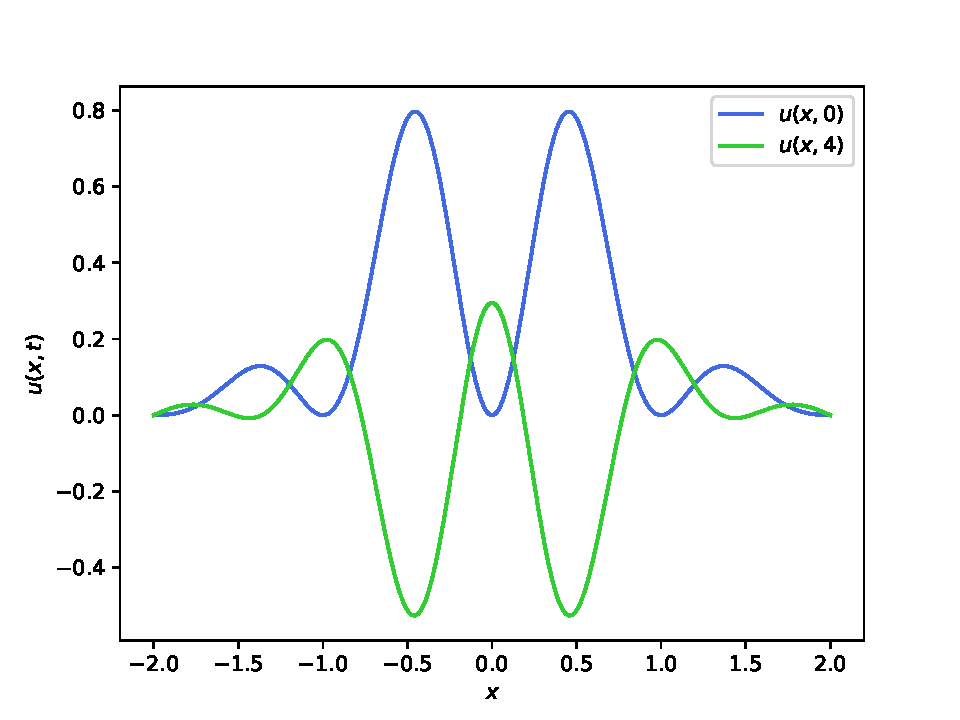
\includegraphics[width=0.85\linewidth]{plots/part2f_sol.pdf}\label{fig:part2f_sol}}\hspace{0mm}
\caption{Sine-Gordon equation solved on $x \in [-2,2]$ and $t \in [0,4]$ with homogeneous Dirichlet conditions and initial condition $u(x,0)=\sin(\pi x)^2 \mathrm{e}^{-x^2}, u_t(x,0) = \sin{(\pi x)^4e^{-x^2}}$. The numerical solution is calculated using RK4 with $M=350$ and $N=500$. Figure (a) shows a 3d-plot of the numerical solution and (b) shows the solution at time $t=0$ and $t=4$.}
\end{figure}

From task \textbf{b)}, the energy is on the form 
\begin{equation*}
    E(t) = \int_{-2}^2 \left(\frac{1}{2}u_t^2(x,t) + \frac{1}{2}u_x^2(x,t)+ 1 -\cos{(u(x,t))}\right) \mathrm{d}x,
\end{equation*}
and fulfills the relation

\begin{equation*}
    E(t) = E(0) + \int_0^t \left( u_t(2,t')u_x(2,t')-u_t(-2,t')u_x(-2,t') \right) \mathrm{d}t'.
\end{equation*}
The Dirichlet boundary conditions yield $u_t(-2,t)=u_t(2,t)=0$, which means that the energy is conserved in the system. From numerical calculations, shown in figure \ref{fig:part2f-energy-form}, it is clear that the energy oscillates around a fixed value until $t=4$, when the solution is anti-symmetric with regards to the starting position and the energy reaches its initial energy $E(0)$ precisely. 

\begin{figure}[t]
    \centering
    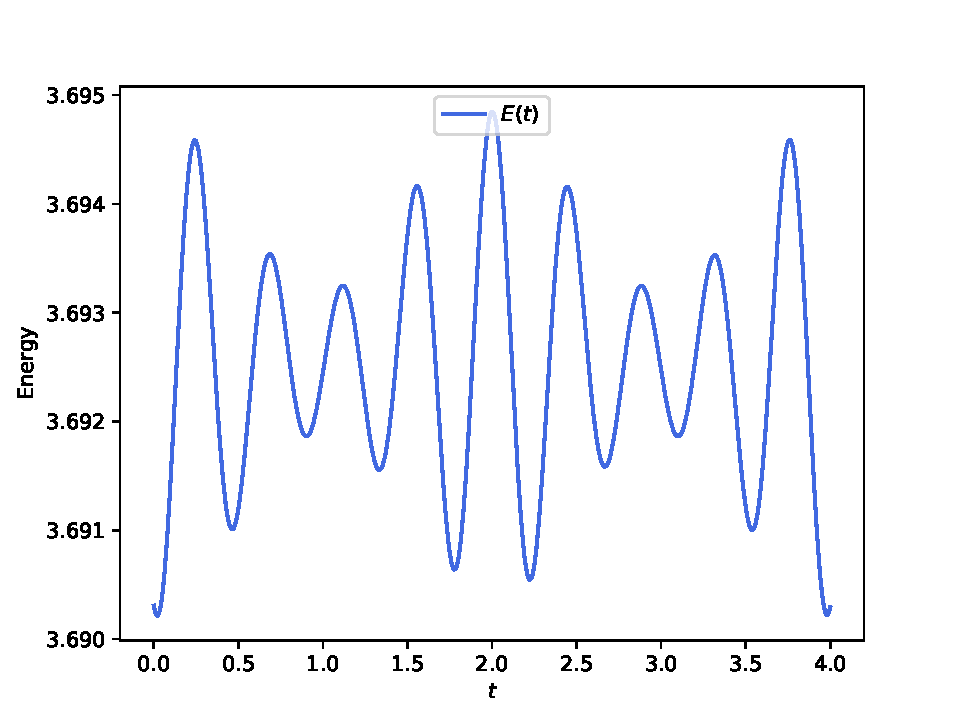
\includegraphics[width = 0.85\linewidth]{plots/part2f_energy.pdf}
    \caption{The energy of the Sine-Gordon equation solved on $x \in [-2,2]$ and $t \in [0,4]$ with homogeneous Dirichlet conditions and initial condition $u(x,0)=\sin(\pi x)^2 \mathrm{e}^{-x^2}, u_t(x,0) = \sin{(\pi x)^4e^{-x^2}}$, is plotted as a function of time. The numerical solution is calculated using RK4 with $M=350$ and $N=500$.} 
    \label{fig:part2f-energy-form}
\end{figure}

The integral in the energy-relation at a given time step, is calculated with Gaussian quadrature \textcolor{blue}{La til "quadrature" i koden også, siden denne gir Gaussisk. Kan se på forskjellen.}\textcolor{red}{QUADPACK} \textcolor{blue}{La til en kommentar om interpolasjon: Ok?}. More precisely, after the quantities in the integrand are found, the values in the discrete grid points are interpolated using cubic interpolation, before the integral of the resulting function is approximated with Gaussian quadratue. The quantities $u_t$ and $u$ are found by integrating with the RK4 or the RKN-34 method, while the spatial derivative $u_x$ is found by differentiation. By using a central difference approximation, explained in section \ref{section_2.2}, the truncation error in $x$ is of second order. In order to achieve second order accuracy at the boundaries, the formula \eqref{Second-order-first-der-B.C}, as introduced in Task 1, is used. Hence, the approximate derivative is given by 

\begin{equation}
    (\boldsymbol{V}^n)' = \frac{1}{2h} 
    \begin{pmatrix}
    -3 & 4 & -1 & &\\
    -1 & 0 & 1 & & \\
    &\ddots & \ddots & \ddots& \\
    & &-1 & 0 & 1 \\
    & & 1 & -4 & 3
    \end{pmatrix}
    \boldsymbol{V}^n,
\end{equation}
where $\boldsymbol{V} = [V_0, V_1, \dots, V_{M+1}]^T$ is the numerical solution at time step $t=t_n$.

The normalized energy difference $\Delta E = \frac{|E(4)-E(0)|}{E(0)}$, hereby denoted the \textit{energy difference}, is calculated for different types of refinement, with both the RK4 and RKN-34 method. $(h=ck)$-refinement, or rather $(N=cM)$-refinement, is performed, for different values of the constant $c$. The $c$ values chosen are $c=\{1.5, 2.0, 2.5\}$ and the $M$ values are doubled for each refinement in the range $M=32$ to $M=2048$. The corresponding plots are shown in figure \ref{fig:part2f_Eref}. From the figure it is observed that the energy difference is smaller for the RK4 than the RKN-34 method, especially for large values of $M$ and $N$ \textcolor{red}{Dette endres litt når man bruker "quadrature" (Gaussisk). Og, er ikke dette en motsigelse mot energien som ble plottet tidligere, der vi skrives at energien er lik i t = 0 som t = 4?}. Furthermore, it looks like the difference between the two methods decreases with larger values of the constant $c$. This is due to a higher resolution grid along in the time direction, and hence, greater accuracy.  

\begin{figure}[!t]
  \centering
  \subfloat[$c=1.5$]{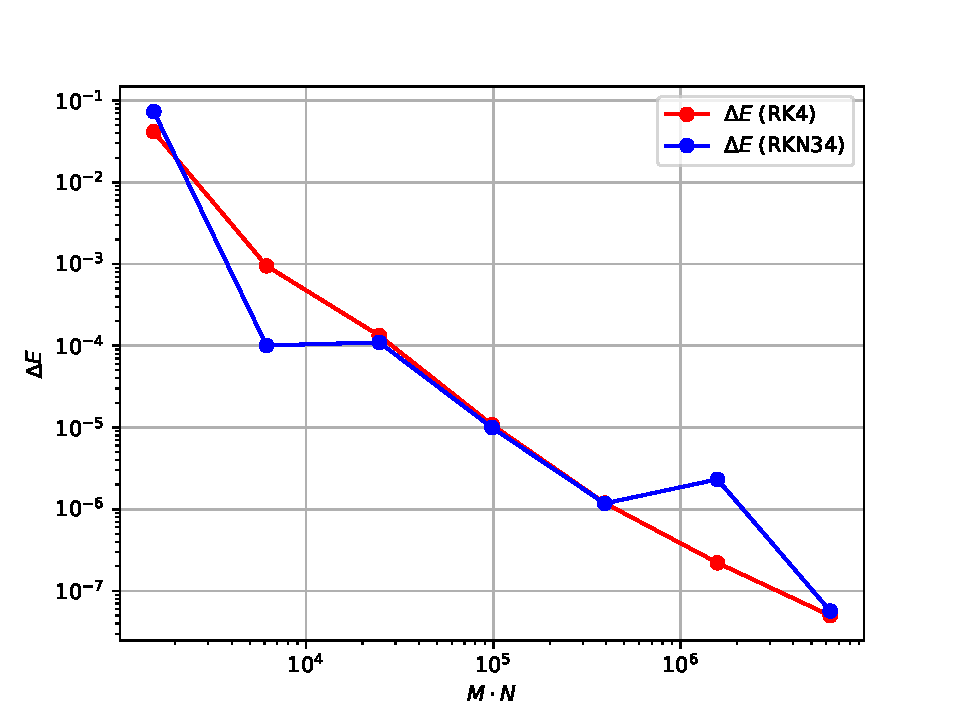
\includegraphics[width=0.5\textwidth]{plots/part2_Eref_a.pdf}\label{fig:Eref_a}}
  \hfill
  \subfloat[$c=2$]{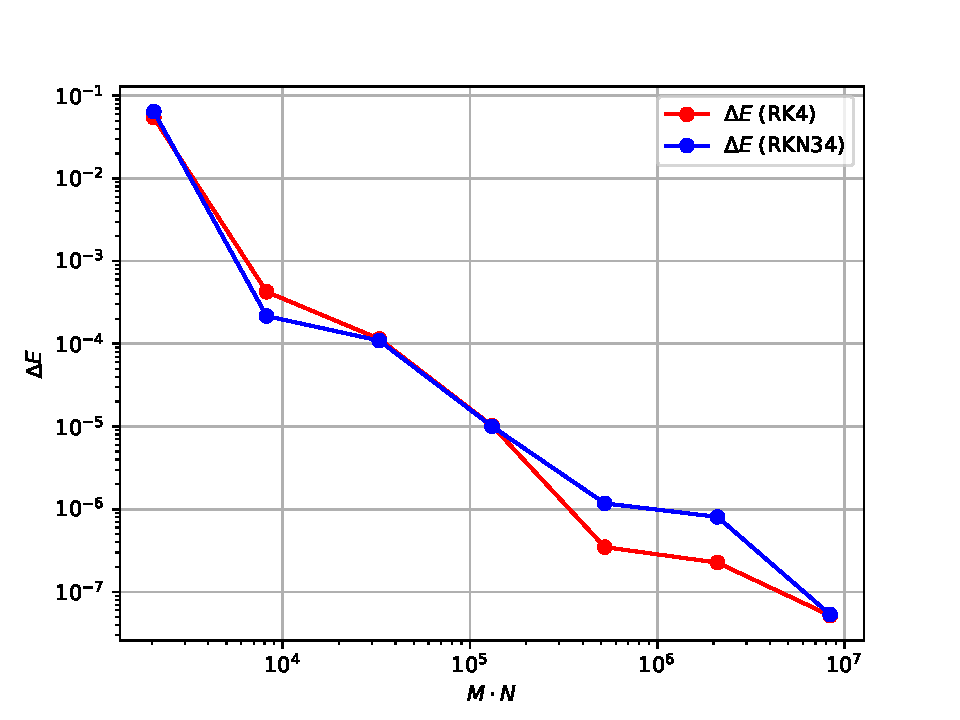
\includegraphics[width=0.5\textwidth]{plots/part2_Eref_b.pdf}\label{fig:Eref_b}}
  \hfill
  \subfloat[$c=2.5$]{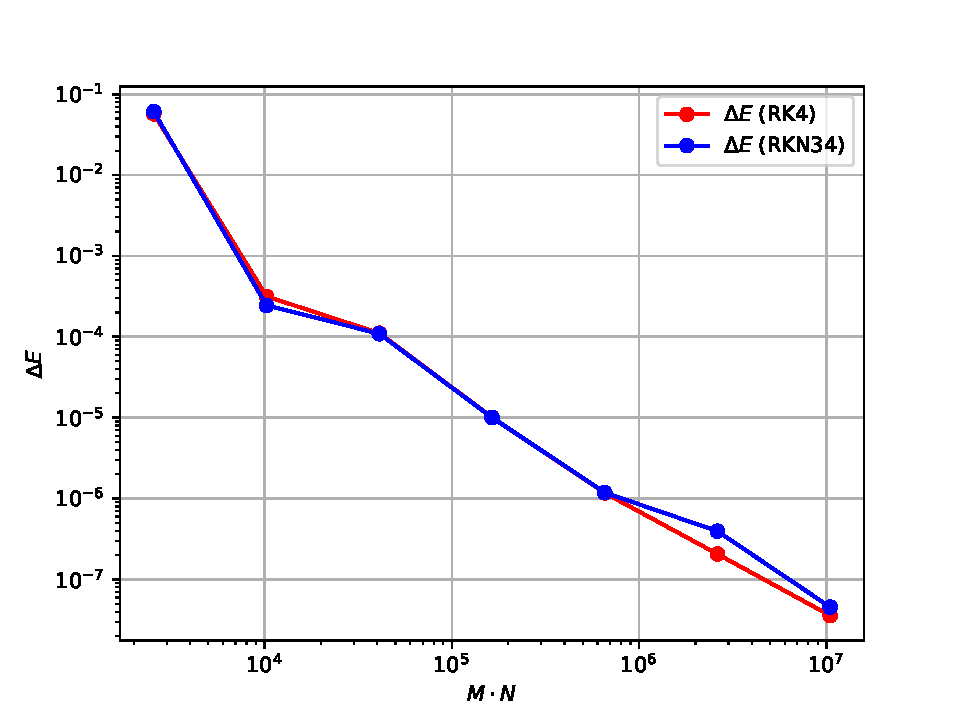
\includegraphics[width=0.5\textwidth]{plots/part2_Eref_c.pdf}\label{fig:Eref_c}}
  \caption{Sine-Gordon equation solved on $x \in [-2,2]$ and $t \in [0,4]$ with homogeneous Dirichlet conditions and initial condition $u(x,0)=\sin(\pi x)^2 \mathrm{e}^{-x^2}, u_t(x,0) = \sin{(\pi x)^4e^{-x^2}}$. The energy difference is calculated for $(N=cM)$-refinement with $c=\{1.5,2.0,2.5\}$ for both the RK4 and RKN-34 methods.}
  \label{fig:part2f_Eref}
\end{figure}

Next, the computation time for the RK4 and RKN-34 methods is compared. To this end, consider a wider range of $M$ values, doubling for each refinement, starting at $M=32$ until $M=4096$. First, $(N=cM)$-refinement, with $c=2$, is performed. The computation times for both methods are shown in figure \ref{fig:time_a} as a function of the number of degrees of freedom in the system, i.e $M \cdot N$. The two methods look almost equally efficient, except for some values where RK4 is slightly slower. Next, the grid is refined in such a way that $N=15000$, i.e. constant at a large value, and the $M$ values are increased. The computation times are displayed in figure \ref{fig:time_b}. A slightly larger difference between the integrators is present, where the RK4 method is the slowest of the two. The reason why RK4 is slower may be due to the increased number of function evaluations of $F$.

The results show that RK4 conserves energy better, but is a bit slower, compared to the RKN-34 method. This is a usual trade-off in numerics where one must choose between accuracy and efficiency. When one wants to conclude on which method is superior, the specific usage must be taken into account. Therefore, one cannot conclude that either of the two integrators is better in all cases, but one has to prioritize which qualities are most important in each specific case. \textcolor{red}{Noe mer vi har misset i konklusjonen?}

\begin{figure}
  \centering
  \subfloat[]{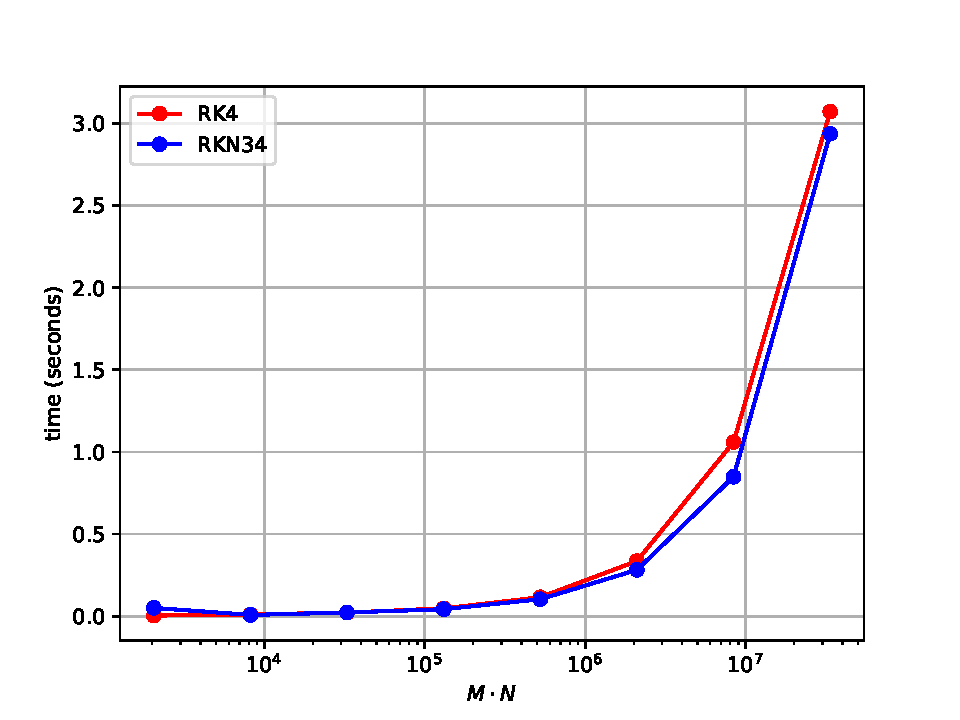
\includegraphics[width=0.85\textwidth]{plots/part2_time_a.pdf}\label{fig:time_a}}\hspace{0mm}
  \subfloat[]{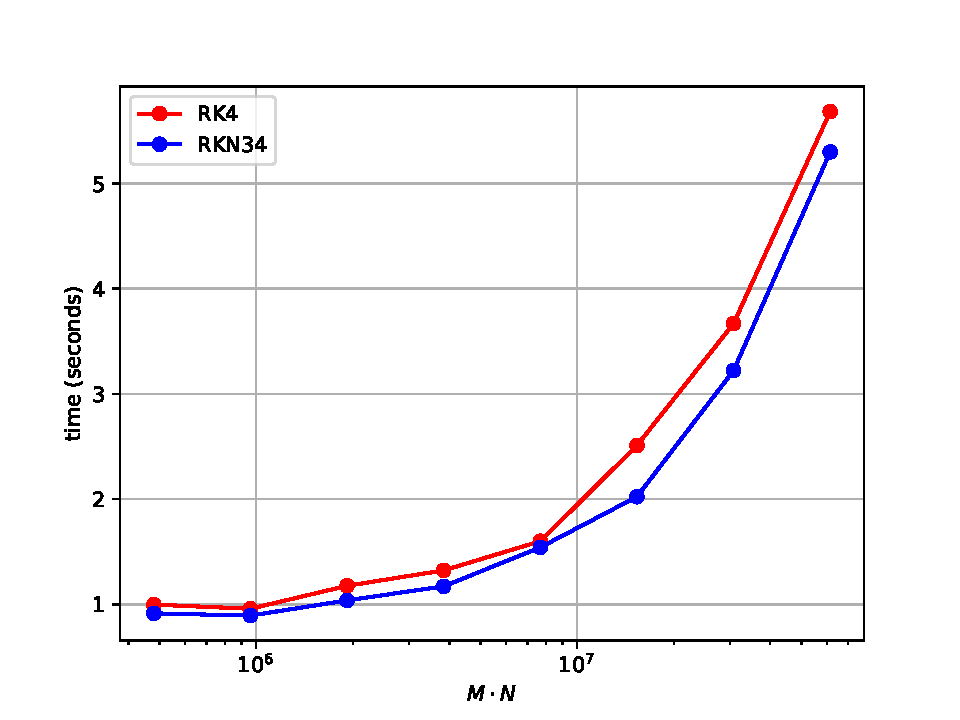
\includegraphics[width=0.85\textwidth]{plots/part2_time_b.pdf}\label{fig:time_b}}\hspace{0mm}
  \caption{Sine-Gordon equation solved on $x \in [-2,2]$ and $t \in [0,4]$ with homogeneous Dirichlet conditions and initial condition $u(x,0)=\sin(\pi x)^2 \mathrm{e}^{-x^2}, u_t(x,0) = \sin{(\pi x)^4e^{-x^2}}$. The computation times for both RK4 and RKN-34 are calculated with $(N=2M)$-refinement, and $N=15000$ with $M$-refinement, as shown in (a) and (b) respectively.}
  \label{fig:part2f_time}
\end{figure}



\newpage
\ 
\newpage